\chapter{Extra Information}
\section{Use Case Diagram} \label{UseCase}
%The appendices contain information that is peripheral to the main body of the report. Information typically included in the Appendix are things like tables, proofs, graphs, test cases or any other material that would break up the theme of the text if it appeared in the body of the report. It is necessary to include your source code listings in an appendix that is separate from the body of your written report (see the information on Program Listings below).
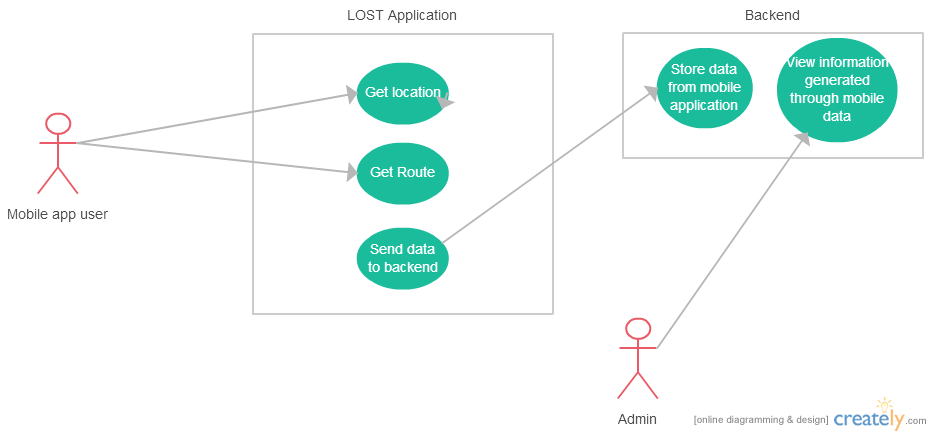
\includegraphics[scale=0.40]{UseCase}

\newpage

\section{Component Diagram}
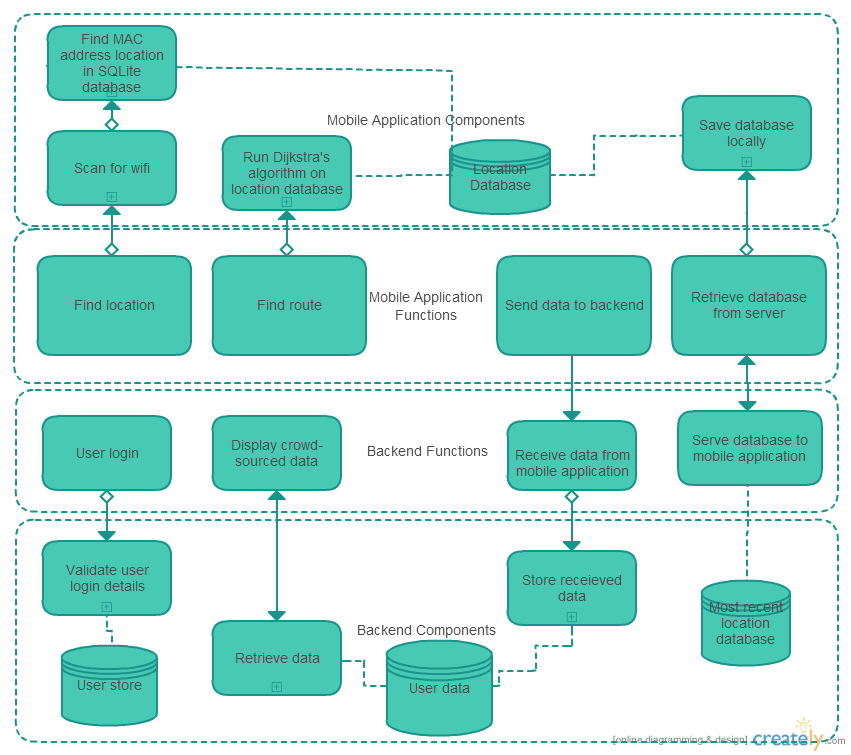
\includegraphics[scale=0.50]{ComponentDiagram}

\newpage
\section{Class Diagram - LOST}
\includegraphics[scale=0.40]{lostclass}

\newpage
\section{Class Diagram - FOUND}
\includegraphics[scale=0.60]{foundclass}

\newpage
\section{Class Diagram - Ruby Controllers}
\includegraphics[scale=0.60]{rubycontrollers}

\section{Class Diagram - Ruby Models}
\includegraphics[scale=0.50]{rubymodels}